\documentclass[a4paper,12pt,titlepage]{article}

\usepackage{listings}
\usepackage{amsmath}
\usepackage{amssymb}
\usepackage{amsthm}
\usepackage{graphicx}
\usepackage{hyperref}
\usepackage{parskip}
\usepackage{pdfpages}

\setlength{\parindent}{15pt}
\hypersetup{colorlinks=true,linkcolor=green}

\begin{document}

\title{Network Security Class \\ Lab Session 2}
\author{Stefano Zanella - 621796}
\date{July 2013}

\maketitle

\section{Assignment}
Experiment with the encoding, transmission and decoding in various realizations
of the UEC, BSC, AWGN channels and for different parameters. Evaluate
quantitatively and illustrate with plots and graphs:

\begin{enumerate}
  \item the reliability (in terms of Bob's bit error rate on the secret message) and
        the secrecy (both in terms of Eve's bit error rate and information on the
        secret message) for the binary symmetric channel, over a wide range of bit
        error rates of the channels.

  \item the reliability (in terms of Bob's bit error rate on the secret message) and
        the secrecy (both in terms of Eve's bit error rate and information on the
        secret message) for the additive white Gaussian noise, over a wide range of
        signal to noise ratios of the channels.
\end{enumerate}

Discuss your results, in relationship with the channel secrecy capacity.

\newpage

\section{Uniform Error Channel}

We start with the ideal case of a UEC. The given model sets a codeword length
$l_x$ of $7$ bits; also it defines two different values for the number of
errors that the legitimate and eavesdropper channels make during transmission,
which are respectively $n_{err_B} = 1$, $n_{err_E} = 3$.

\subsection*{Theoretical analysis}
From given parameters, we can derive the other variables that let us fully characterize
the model, thus allowing for precise analysis of secrecy metrics. \\
We start from calculating the value of $N_{y|x}$ and $N_{z|x}$, which are the
cardinalities of the sets $T_{y|x}(a)$ and $T_{z|x}(a)$ that determine the
possible messages Bob and Eve can receive given a determined $a \in
\mathcal{X}$ and their respective number of possible errors. Using this
definition, it's easy to retrieve the two values: that is, given $n_{err_B}$
and a generic 7 bit codeword $a \in \mathcal{X}$, on the other
side Bob can receive all 7 bit codewords containing $0$ up to $n_{err_B}$
errors. This value is represented as:
\[N_{y|x} = \sum_{i = 0}^{n_{err_B}} {7 \choose i} = 8\]
With the same approach we say that
\[N_{z|x} = \sum_{i = 0}^{n_{err_E}} {7 \choose i} = 64\]

That said, we can calculate the number of possible secret messages. We know
from the theory of UECs and general physical layer secrecy that
\[\left|\mathcal{M}\right| \leq
\frac{\left|\mathcal{Y}\right| / N_{y|x}}{\left|\mathcal{Z}\right| / N_{z|x}}
= \frac{N_{z|x}}{N_{y|x}} = 8\]
which leads to
\[l_u = \log_2 8 = 3\]

That is, we can use $3$ out of the $7$ available bits to send secret
information. This means we can achieve a secrecy rate of:
\[ R_s = \frac{\log_2 |\mathcal{M}|}{n} = \frac{l_u}{l_x} = \frac{3}{7} \simeq 0.4286 \]

Also, we can say that the channel has a secrecy capacity of:
\begin{align*}
C_s &= I(x, y) - I(x, z) \\
    &= (H(x) - H(x|y)) - (H(x) - H(x|z)) \\
    &= H(x|z) - H(x|y) \\
\end{align*}
which can be described, in the case of a UEC, as:
\begin{align*}
C_s &= - \log_2 \frac{2^{l_x}}{N_{z|x}} + \log_2 \frac{2^{l_x}}{N_{y|x}} \\
    &= \log_2 \frac{N_{z|x}}{2^{l_x}} - \log_2 \frac{N_{y|x}}{2^{l_x}} \\
    &= \frac{\log_2 N_{z|x} - \log_2 N_{y|x}}{l_x} \\
    &= \frac{\log_2 {\frac{N_{z|x}}{N_{y|x}}}}{l_x} \\
    &= \frac{\log_2 8}{7} = \frac{3}{7} \simeq 0.4286
\end{align*}

This means that in the case of an UEC we can aim at transmitting secret
information filling the channel secrecy capacity.

\subsection*{Designing the encoder and decoder}
At this point we've defined what are the achievable secrecy metrics in theory;
we still need to actually design the encoder and the decoder so that we can do
an actual simulation of secure transmission over the UEC. \\
We recap the basic features of (secure) physical layer encoder and decoder:
\begin{itemize}
  \item The encoder is probabilistic, defined by $P_{x|u}(a|d) \; a \in
  \mathcal{X}, d \in \mathcal{M}$
  \item The decoder is deterministic, defined by the function \\
  $\hat{u} = D(y) \; D: \mathcal{Y} \rightarrow \mathcal{M}$
  \item The encoding/decoding process is \textbf{correct}: $P[\hat{u} \neq u] =
  0$
  \item $u$ is independent of the eavesdropped $z$ (\textbf{secrecy}
  requirement).
\end{itemize}

We can divide the design process in two steps: coding for \emph{reliability}
(correctness) and coding for \emph{secrecy}. In the first step we design the
code $\mathcal{x'}$ so that it obeys to the property that each codeword $a \in \mathcal{X'}$
maps to a subset $T_{y|x}(a) \subset \mathcal{Y}$ and $\forall (a_1, a_2) \in
\mathcal{X'}, a_1 \neq a_2 T_{y|x}(a_1) \cap T_{y|x}(a_2) = \emptyset$. In the
second step, instead, we refine the result of the preceding step so that the
eavesdropper message space $\mathcal{Z}$ is filled in such a way to make
indistinguishable which the original message $d \in \mathcal{M}$ was (from an
attacker's perspective).

To obtain the first property, since $n_{err_B} = 1$ we can rely on Hamming codes;
for a given message
$a$, its corresponding subset in $\mathcal{Y}$ must contain it plus all
messages with Hamming distance at most $n_{err_B}$ from it. \\
Also, we need to make every subset to be at distance $> 2n_{err_B}$ to achieve
correctness. Since we are talking about binary codes, this translates into
saying that the minimum distance between subsets is $2n_{err_B} + 1 = 3$.
A code that satisfies this property is \texttt{Hamming(7,4)}; it allows not
only to define disjoint subsets over $\mathcal{Y}$, but to actually define a
\emph{partition} of $\mathcal{Y}$.

That said, we can now consider code secrecy with respect to the eavesdropper.
As already said, such a code should fill the eavesdropper message space
$\mathcal{Z}$. We already saw that $N_{z|x} = 64$; this means that the $Z$ set
is partitioned into $2^{l_x}/N_{z|x} = 2$ subsets. \\
A way to define these two subsets is to consider messages which are one the
complement of the other and put them in different subsets. That is, messages at
$d_H = 7$ belong to different subsets. It's easy to see how this is an
equipartition of $\mathcal{Z}$, thus obeying to the properties of the UEC. \\
That said, we need a way to design the encoder so that for every message $d \in
\mathcal{M}$ there is an equal probability that its encoding belongs to each of
the two subsets. This can be done as follows:
\begin{itemize}
  \item pick a generic message $u = u_1 \; u_2 \; u_3$ and choose a bit $b$ at
  random: $b \sim \mathcal{U}(\mathbf{B})$.
  \item let
  \[
    v = 
    \begin{cases}
      b|u & \text{if } b = 0 \\
      b|\bar{u} & \text{if } b = 1
    \end{cases}
  \]
  \item encode $v$ with \texttt{Hamming(7,4)}
\end{itemize}
It turns out that the two choices for $v$ are complementary, and so are the
\texttt{Hamming(7,4)} codewords for them. This means that:
\begin{itemize}
  \item the encoder is probabilistic as requested:
  \[
    P_{x|u}(a|d) = 
    \begin{cases}
      1/2 & \text{if } a \in T_{x|u}(d) \\
      0   & \text{otherwise}
    \end{cases}
  \]
  \item the decoder is deterministic: since it has $n_{err_B} = 1$, the
  \texttt{Hamming(7,4)} code allows for correct recovery of the original
  message $x$. Then, the decoder can just discard the $3$ bits prepended by the
  Hamming encoder and retrieve $v$. At this point, it can look at the first bit
  $b$ and decode:
  \[
    \hat{u} = 
    \begin{cases}
      v_2 \; v_3 \; v_4 & \text{if } b = 0 \\
      \overline{v_2 \; v_3 \; v_4} & \text{if } b = 1
    \end{cases}
  \]
  \item eavesdropper message space is covered by each and every message $d \in
  \mathcal{M}$; furthermore, each of its subsets is disjoint from each other.
  \item legitimate receiver message space is divided into disjoint subsets.
\end{itemize}
So, mathematically, the transmission with the designed encoder is both
\emph{reliable} and \emph{secure}. We now need to actually measure secrecy and
reliability with the Matlab simulation.

\subsection*{Transmission simulation}
The simulation is performed by \texttt{UECscript.m}. It accepts two parameters:
a number of trials and a number representing how many times to repeat that
number of trails in a cumulative way. It basically simulates
$\text{trials} \cdot \text{split}$ transmissions over the UEC, counting the number of errors made by
the legitimate receiver and the eavesdropper. Then, every \texttt{trials}
transmissions, it calculates the BER for
the two transmission ends and print an histogram representing residual information
on $u$ given a particular $z$ for every codeword $x$, as well as
information about messages, joint and mutual entropies.

We start by observing that we need to perform a certain number of transmissions
before reaching the bounds given by the statistical model. In particular, this
can be noticed when looking at the measured conditional entropy between $u$ and
$z$. Looking at Figure~\ref{fig:uec_Hudz} we see that we approach asymptotically the
theoretical result of statistical independence between $u$ and $z$ (which means
$H_{u|z} = l_u = 3$); to obtain a good approximation, we need to consider at
least 8-10000 samples (to have $\delta \sim 2\%$). \\
\begin{figure}[h]
  \centering
  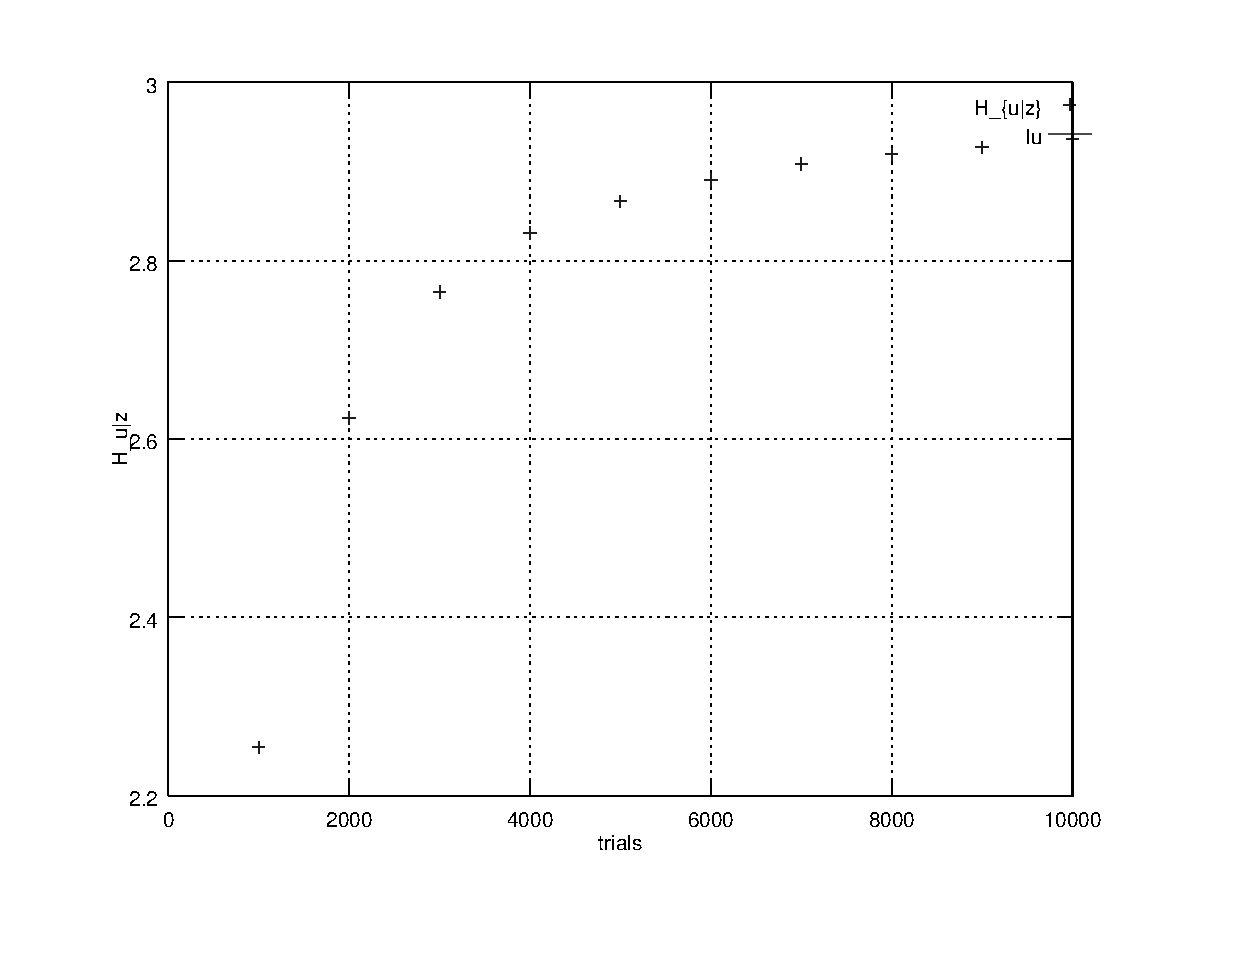
\includegraphics[scale=0.8]{uec_Hudz.eps}
  \caption{$H_{u|z}$ vs. number of trials}
  \label{fig:uec_Hudz}
\end{figure}

The same result can be observed comparing the histograms depicting conditional
entropy for every codeword fixed $z=0$ with different number of trials. That
is, if we compare Figure~\ref{fig:uec_1000}, \ref{fig:uec_5000} and
\ref{fig:uec_10000}, we see that with only 1000 experiments there are certain
codewords that let leak 2 bits of the original message. This is clearly not a
flaw of the model, but it rather points an insufficient amount of data; this is
confirmed by looking at what happens with 5000 and 10000 experiments; we see
that the distribution among the codewords tends to become flat and within 0.25
bit from the theoretical result.

\begin{figure}[h]
  \centering
  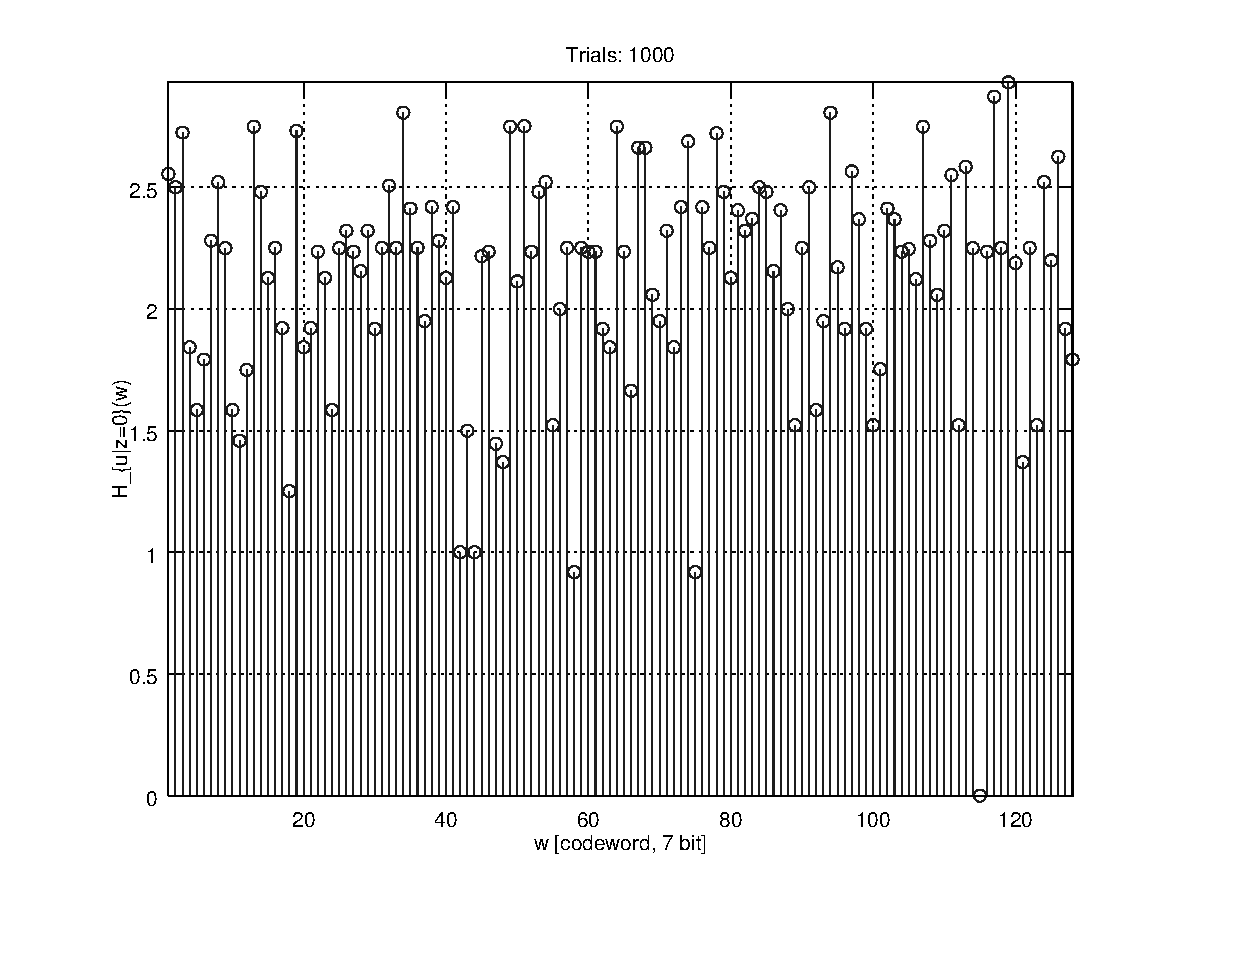
\includegraphics[scale=0.8]{uec_1000.eps}
  \caption{$H_{u|z=0}$ with 1000 trials}
  \label{fig:uec_1000}
\end{figure}

\begin{figure}[h]
  \centering
  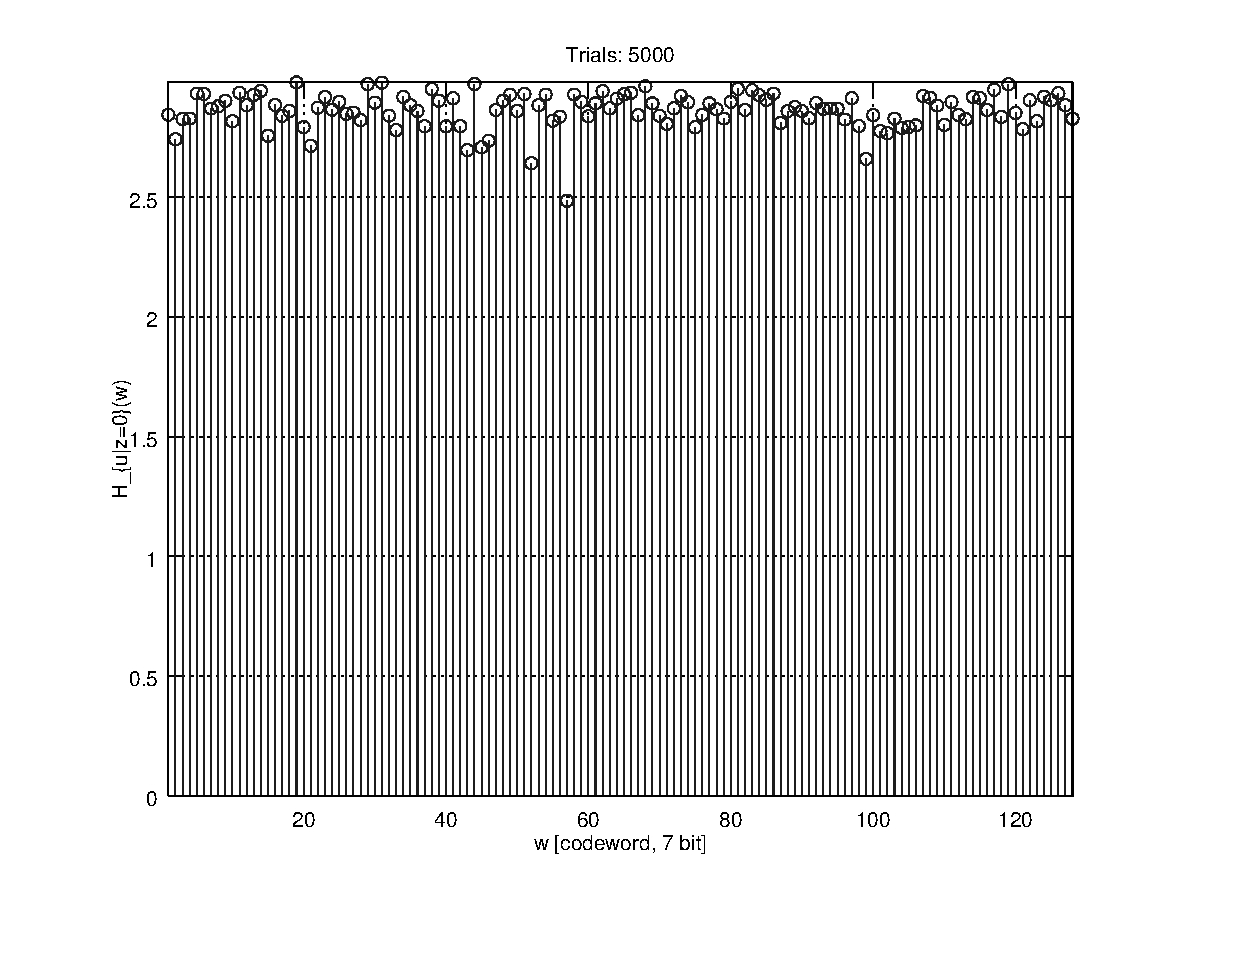
\includegraphics[scale=0.8]{uec_5000.eps}
  \caption{$H_{u|z=0}$ with 5000 trials}
  \label{fig:uec_5000}
\end{figure}

\begin{figure}[h]
  \centering
  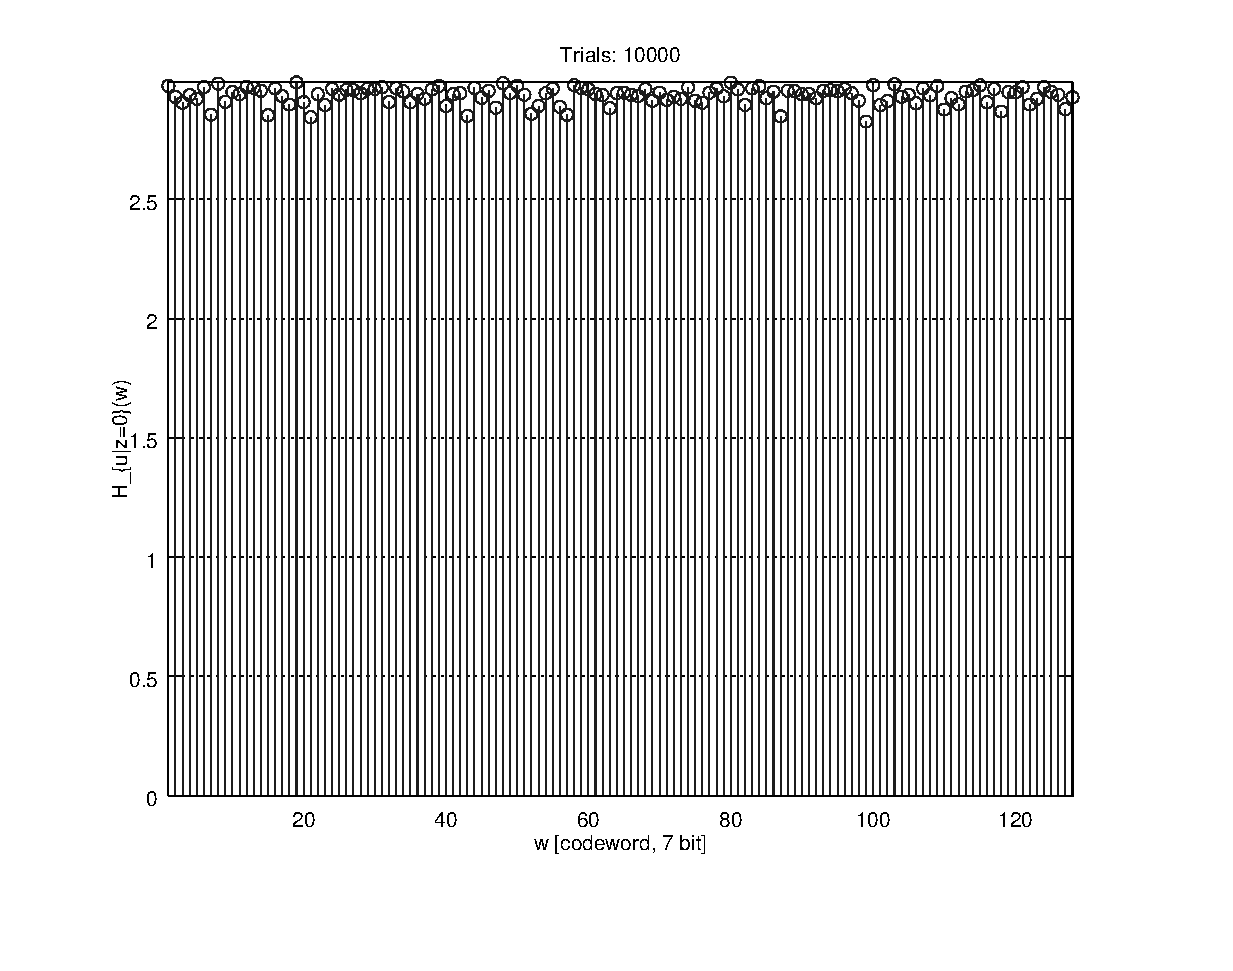
\includegraphics[scale=0.8]{uec_10000.eps}
  \caption{$H_{u|z=0}$ with 10000 trials}
  \label{fig:uec_10000}
\end{figure}

At the same time, we can see another interesting result. Conversely from the
case of conditional entropy, if we plot the BER against the number of
experiments for both the legitimate receiver and the eavesdropper as in
Figure~\ref{fig:uec_ber}, we see that
no matter how many experiments we do:
\begin{itemize}
  \item The BER at the legitimate receiver is always $0$
  \item The BER at the eavesdropper fluctuates tightly around $0.5$
\end{itemize}
This is an expected result and proves the design of the encoder is done right.
In fact, the first observation tells us that the codec achieves \emph{correctness}. This is
expected since we used an 1-bit error-correction code and the legitimate
receiver can make \emph{at most} 1 error. \\
Instead, the second observation tells us that we achieve the goal of confusing
the attacker as much as possible: in fact, achieving a BER of $0.5$ means that,
for every received bit, the attacker has no clue if it has been corrupted during
transmission or not, and so he has no better choice than randomly guessing the
eavesdropped secret message.

\begin{figure}[h]
  \centering
  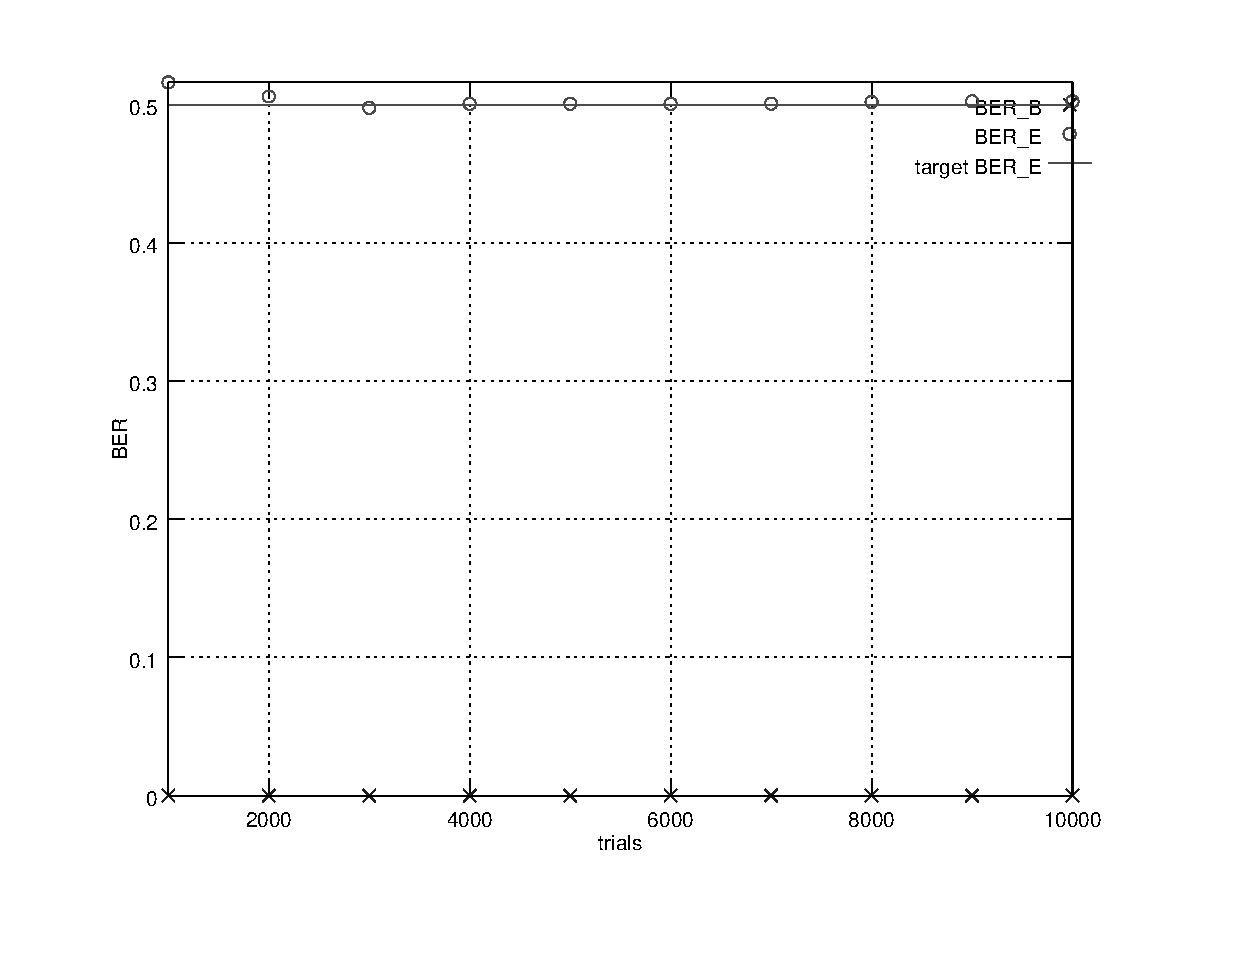
\includegraphics[scale=0.8]{uec_ber.eps}
  \caption{BER for E and B over a UEC}
  \label{fig:uec_ber}
\end{figure}

Also, a note on BER and conditional entropy: we cannot claim we've achieved
(perfect) secrecy just by looking at the BER (it's a necessary condition, but
not sufficient); this is why we also take into
consideration measured conditional entropy between eavesdropped and original
messages. This is because BER is just a global measure over channel's physical
behaviour, but doesn't take into account the \emph{semantic} of the error, that
is, it doesn't provide any information over actual \emph{information}. We can
partially see this in the case of a low number of experiments: while we can
achieve $\text{BER} = 0.5$, we cannot achieve a good conditional entropy. \\
Instead, the notion of perfect secrecy states explicitly that original and
eavesdropped messages must be statistically independent: that is, knowing the
latter doesn't give any advantage over knowledge of the former. By calculating
and plotting conditional entropy we're actually measuring this.

Below, we recap the result of the simulation of 10000 transmissions, as output
by the \texttt{UECscript} function:

\begin{verbatim}
Secrecy capacity = 0.4286
Secrecy rate     = 0.4286
BER at Bob       = 0.00e+00
BER at Eve       = 5.03e-01
-------------------------
H(u)   = 2.9996 bit
H(z)   = 6.9889 bit
H(u,z) = 9.9256 bit
H(u|z) = 2.9367 bit
H(z|u) = 6.9260 bit
I(u;z) = 0.0629 bit
\end{verbatim}

This result will serve as a reference for the models that follow.

\section{Binary Symmetric Channel}
We now look at what happens when we model the channel as a BSC, and see how
secrecy parameters change when error probabilities change.

We use the same encoding scheme as before, so everything said about it still
holds.

\subsection*{Secrecy Capacity}
To start, we try to model a channel as close as possible to the UEC, in terms
of introduced noise. Specifically, we can set the error probabilities
to:\footnote{This doesn't mean there's a strict equivalence
between the values of $\varepsilon_B$ and $\varepsilon_E$, and the error rates
of the UEC. Actually, in the case of the UEC the error rate is considered on
the \emph{whole message}, while the error probability of the BSC is applied
\emph{indipendently for every bit sent}. Though, this simple relation helps
targeting a starting point for the analysis.}
\[
  \varepsilon_B = n_{err_B}/l_x = 1/7 = \simeq 0.14286
\]
\[
  \varepsilon_E = n_{err_E}/l_x = 3/7 = \simeq 0.42857
\]
In this case, it's easy to see that:
\[
  C_s = h_2(\varepsilon_E) - h2(\varepsilon_B) = 0.39356
\]
which is lower than what we achieved with the UEC and corresponds to:
\[
  C_s \cdot l_x = 2.7549 \text{ bit}
\]
that can be concealed in a single message. To achieve a secrecy capacity that
allows to conceal a 3 bit message, we can try to lower $\varepsilon_B$, increase
$\varepsilon_E$, or both. We see that even if we increase $\varepsilon_E$ so to
achieve maximum confusion, i.e. $\varepsilon_E = 0.5$, we can only reach $C_s =
2.8583$. Instead, we can reach our goal by leaving $\varepsilon_E = 0.42857$
and setting $\varepsilon_B = 0.125$, which lead to $C_s \cdot l_x = 3.0916
\text{ bit}$. In this case, the simulation of 10000 transmissions leads to the
following result:
\begin{verbatim}
Metrics with 10000 trials:
Secrecy capacity = 0.4417
Secrecy rate     = 0.4286
BER at Bob       = 1.26e-01
BER at Eve       = 4.88e-01
-------------------------
H(u)   = 2.9989 bit
H(z)   = 6.9923 bit
H(u,z) = 9.9222 bit
H(u|z) = 2.9300 bit
H(z|u) = 6.9233 bit
I(u;z) = 0.0690 bit
\end{verbatim}
Also, in Figure~\ref{fig:bsc_Hudz} it can be seen how conditional entropy is
distributed, as in the case of the UEC.

\begin{figure}[h]
  \centering
  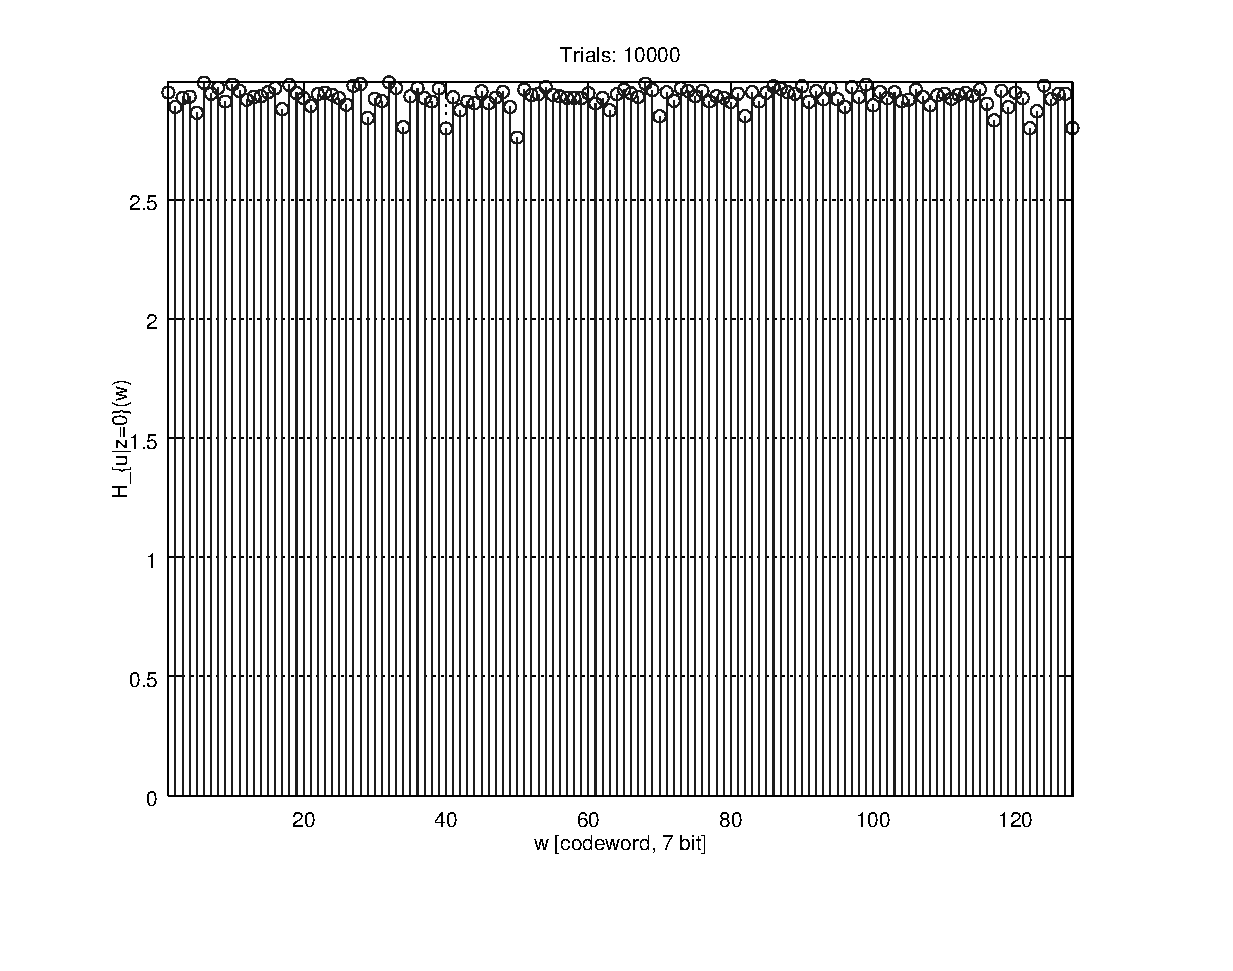
\includegraphics[scale=0.8]{bsc__0_125__0_429__10000.eps}
  \caption{$H_{u|z=0}$ with 10000 trials}
  \label{fig:bsc_Hudz}
\end{figure}

We can make two key observations here:
\begin{itemize}
  \item the model doesn't achieve correctness ($\text{BER}_B > 0$)
  \item albeit the level of secrecy is high both in terms of BER and
  statistical independence of $u$ and $z$, the error probability for
  eavesdropper's channel is very high, meaning the channel is almost unusable
  ($0.5 =$ highest level of confusion).
\end{itemize}

The first one is an important difference from UEC: since every bit transmitted
over a BSC has the same probability $\varepsilon$ of being swapped, we can't be
sure, as in the case of UEC, that the legitimate channel makes at most a fixed
amount of errors. In the particular case of our \texttt{Hamming(7,4)} code, we
can calculate the probability of correctly receiving a message as the
probability of receiving a message with at most 1 error:
\[
  p[\hat{u} = u]_B = (1 - \varepsilon_B)^7 + (1 - \varepsilon_B)^6 \cdot \varepsilon_B
  \simeq 0.44880
\]
which turns out to be less than \%50 percent of the times. \\
On the contrary, on the eavesdropper side, the probability of receiving an
unrecoverable message is:
\begin{align*}
  p[\hat{u} \neq u]_E &= 1 - p[\hat{u} = u]_E \\
  &= 1 - [(1 - \varepsilon_E)^7 + (1 - \varepsilon_E)^6 \cdot \varepsilon_E] \\
  &\simeq 0.99503
\end{align*}
which is extremely high, as already pointed out. \\
We can see the trend of these two functions (isomorph to each other) in
Figure~\ref{fig:decode_probs}.

\begin{figure}[h]
  \centering
  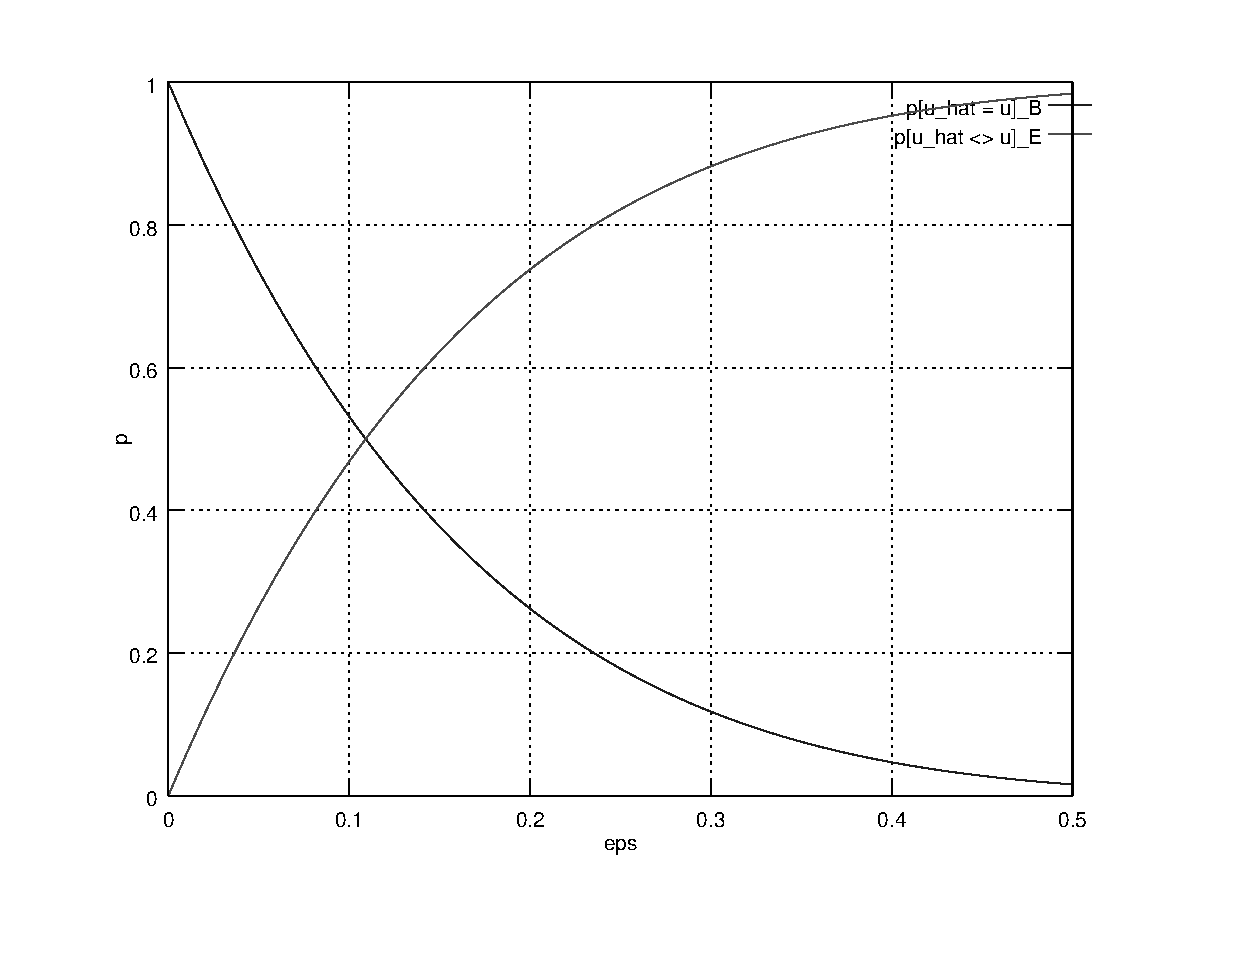
\includegraphics[scale=0.8]{bsc_decoding_probs.eps}
  \caption{Decoding probabilities for the \texttt{Hamming(7,4)} code vs
  $\varepsilon$}
  \label{fig:decode_probs}
\end{figure}

From that, we can also try to see how secrecy capacity evolves when varying
both $\varepsilon_B$ and $\varepsilon_E$. Figure~\ref{fig:bsc_mesh_cs} shows
the 3D curve representing $C_s$ as a function of both variable (when
$\varepsilon_B < \varepsilon_E$, since in the other case the evesdropper would
have an advantage over the legitimate receiver and the roles could be
considered swapped).

\begin{figure}[p]
  \centering
  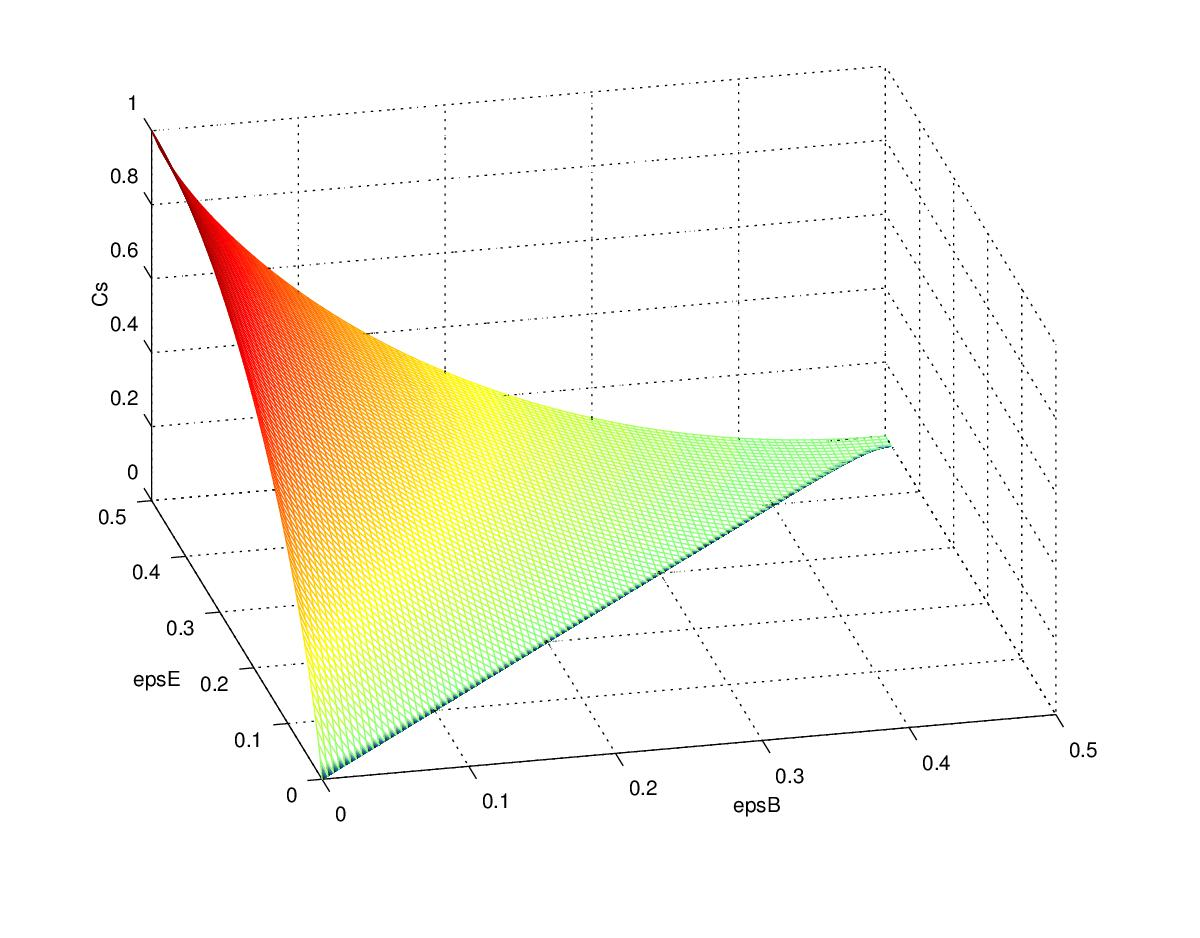
\includegraphics[scale=0.8]{bsc_mesh_cs.jpg}
  \caption{Evolution of secrecy capacity as a function of
  $\varepsilon_B$ and $\varepsilon_E$}
  \label{fig:bsc_mesh_cs}
\end{figure}

From Figure~\ref{fig:bsc_mesh_cs} we can confirm what intuition already pointed
out:
\begin{itemize}
  \item we can't have any form of secrecy when the error probabilities of the
  two channel are equal;
  \item full channel secrecy can be reached only in the (rather theoretical)
  case of $\varepsilon_B = 0, \varepsilon_E = 0.5$;
  \item as error probability for legitimate channel increases, no matter the
  error probability for the eavesdropper, we can only hope to obtain a certain
  amount of secrecy that decreases with the former.
\end{itemize}

That said, we can limit the observation to the cases that give us a secrecy
capacity high enough to conceal the 3 bits we want to send ($C_s > 3/7$).
Figure~\ref{fig:bsc_mesh_cs_3bit} shows the region that satisfies this condition.

\begin{figure}[p]
  \centering
  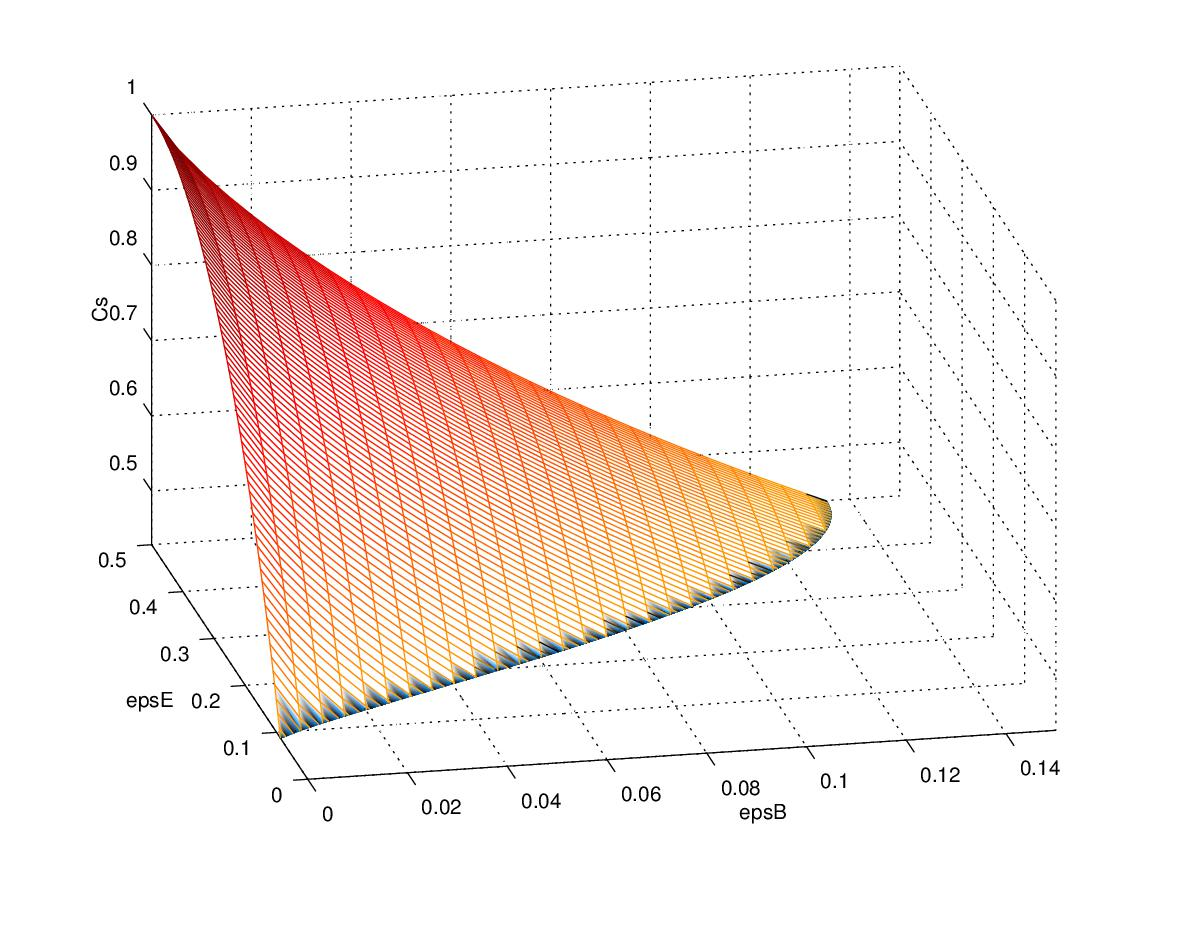
\includegraphics[scale=0.8]{bsc_mesh_cs_3bit.jpg}
  \caption{Evolution of $C_s$ under the constraint $C_s > 3/7$}
  \label{fig:bsc_mesh_cs_3bit}
\end{figure}

From this plot, we can select few points and analyze them more in depth. To
choose them, let's take for granted that we want to send 3 secure bits, and
focus on the following criteria:
\begin{itemize}
  \item points that lead to $R_s = C_s - \varepsilon$
  \item points that lead to $R_s = C_s + \varepsilon$
\end{itemize}
In particular:
\begin{itemize}
  \item $\varepsilon_B = 0.06, \varepsilon_E = 0.22$ ($C_s = 0.43272$)
  \item $\varepsilon_B = 0.12, \varepsilon_E = 0.38$ ($C_s = 0.42868$)
  \item $\varepsilon_B = 0.10, \varepsilon_E = 0.30$ ($C_s = 0.41230$)
  \item $\varepsilon_B = 0.06, \varepsilon_E = 0.22$ ($C_s = 0.31957$)
\end{itemize}

\newpage

\subsection*{Number of experiments}
Before starting the analysis, let's first determine how many transmission to do
per instance of the model. \\
If we plot the BER and the conditional entropies vs. the number of
trials for a fixed value of $\varepsilon_B$ and $\varepsilon_E$ (i.e. $0.1$ and
$0.35$ respectively), we see (Figure~\ref{fig:bsc_ber} and
\ref{fig:bsc_ber}) that:
\begin{itemize}
  \item as in the previous case, the value of BER for both Bob and Eve doesn't
  have direct relationship with the number of trials
  \item the value of conditional entropy still has a relationship with the
  number of trials, but there is somewhat less variation in the range $[5000,
  10000]$ than in the case of UEC.
\end{itemize}

\begin{figure}[p]
  \centering
  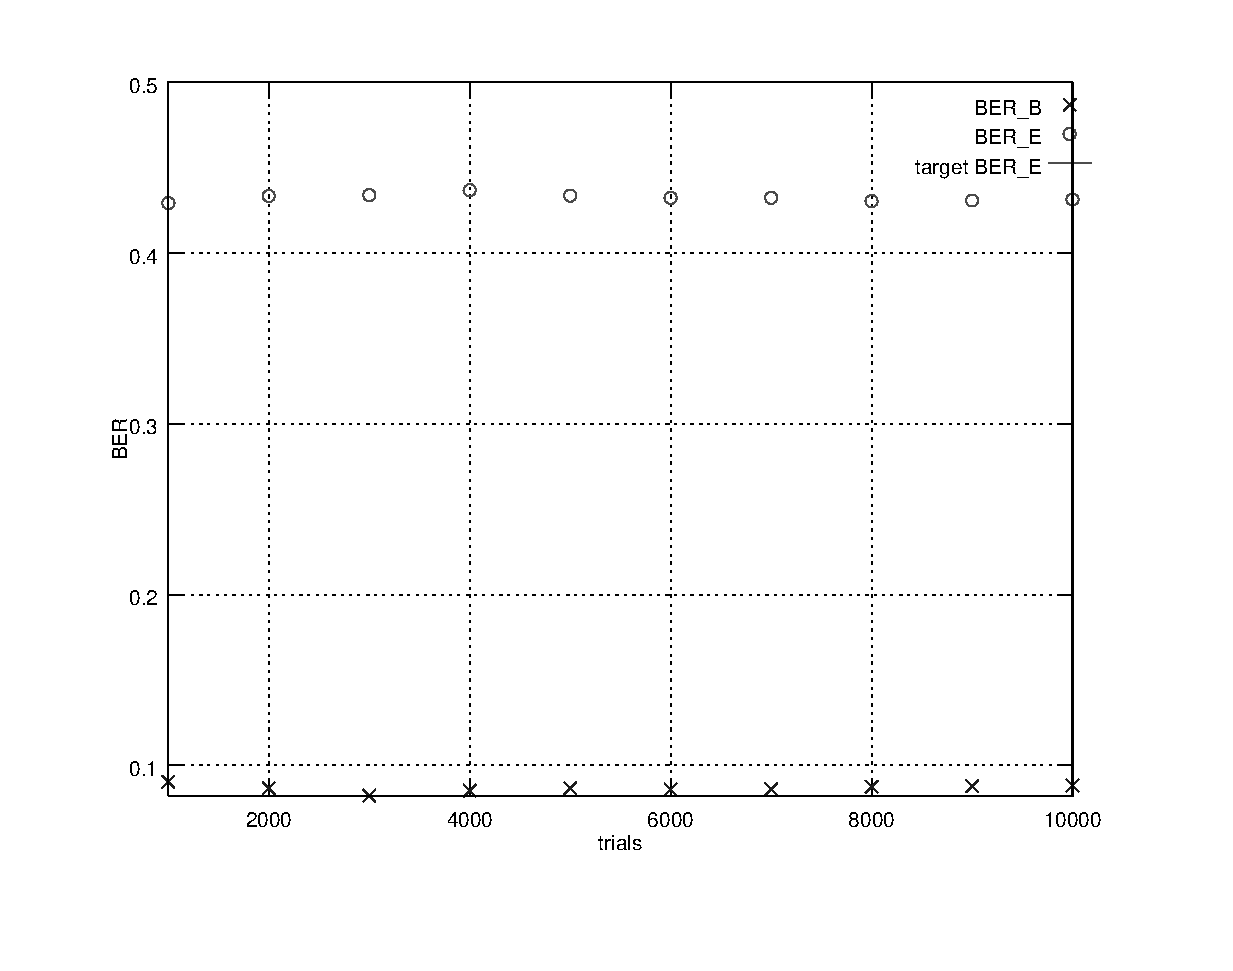
\includegraphics[scale=0.6]{bsc_ber.eps}
  \caption{BER for E and B over a BSC}
  \label{fig:bsc_ber}

  \centering
  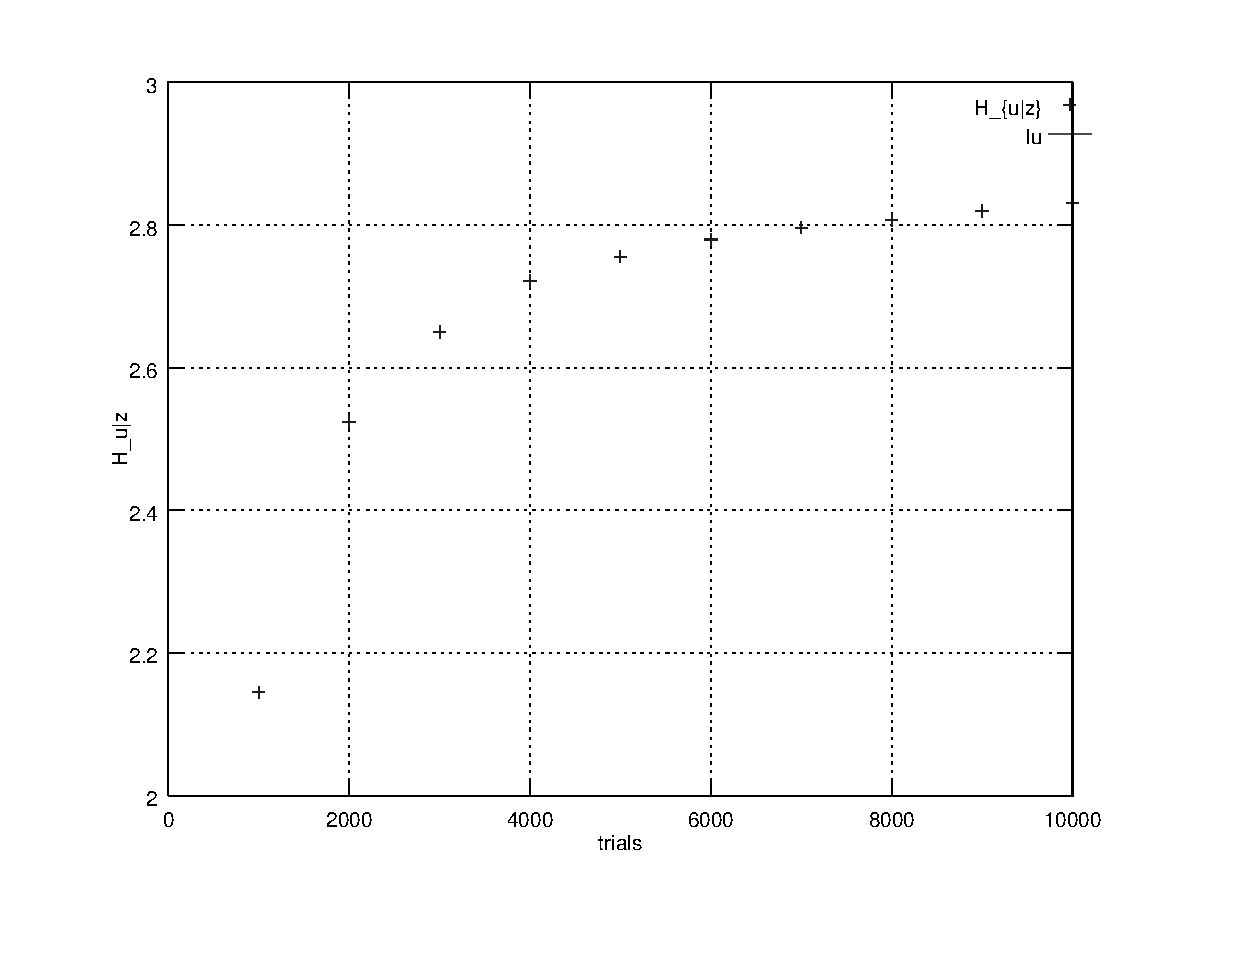
\includegraphics[scale=0.6]{bsc_Hudz.eps}
  \caption{$H_{u|z}$ vs. number of trials}
  \label{fig:bsc_Hudz}
\end{figure}

For these reasons, given that running a simulation with 10000 transmissions is
quite expensive in terms of time, let's just reduce them to 6000.

\newpage

\subsection*{$R_s < C_s$: $\varepsilon_B = 0.06, \varepsilon_E = 0.22$}
The results of the simulation are summarized in Figure~\ref{fig:bsc_0.6_0.22} and
in the following output:
\begin{verbatim}
Metrics with 6000 trials:
Secrecy capacity = 0.4327
Secrecy rate     = 0.4286
BER at Bob       = 3.58e-02
BER at Eve       = 2.75e-01
-------------------------
H(u)   = 2.9994 bit
H(z)   = 6.9468 bit
H(u,z) = 9.0126 bit
H(u|z) = 2.0657 bit
H(z|u) = 6.0131 bit
I(u;z) = 0.9337 bit
\end{verbatim}

\begin{figure}[h]
  \centering
  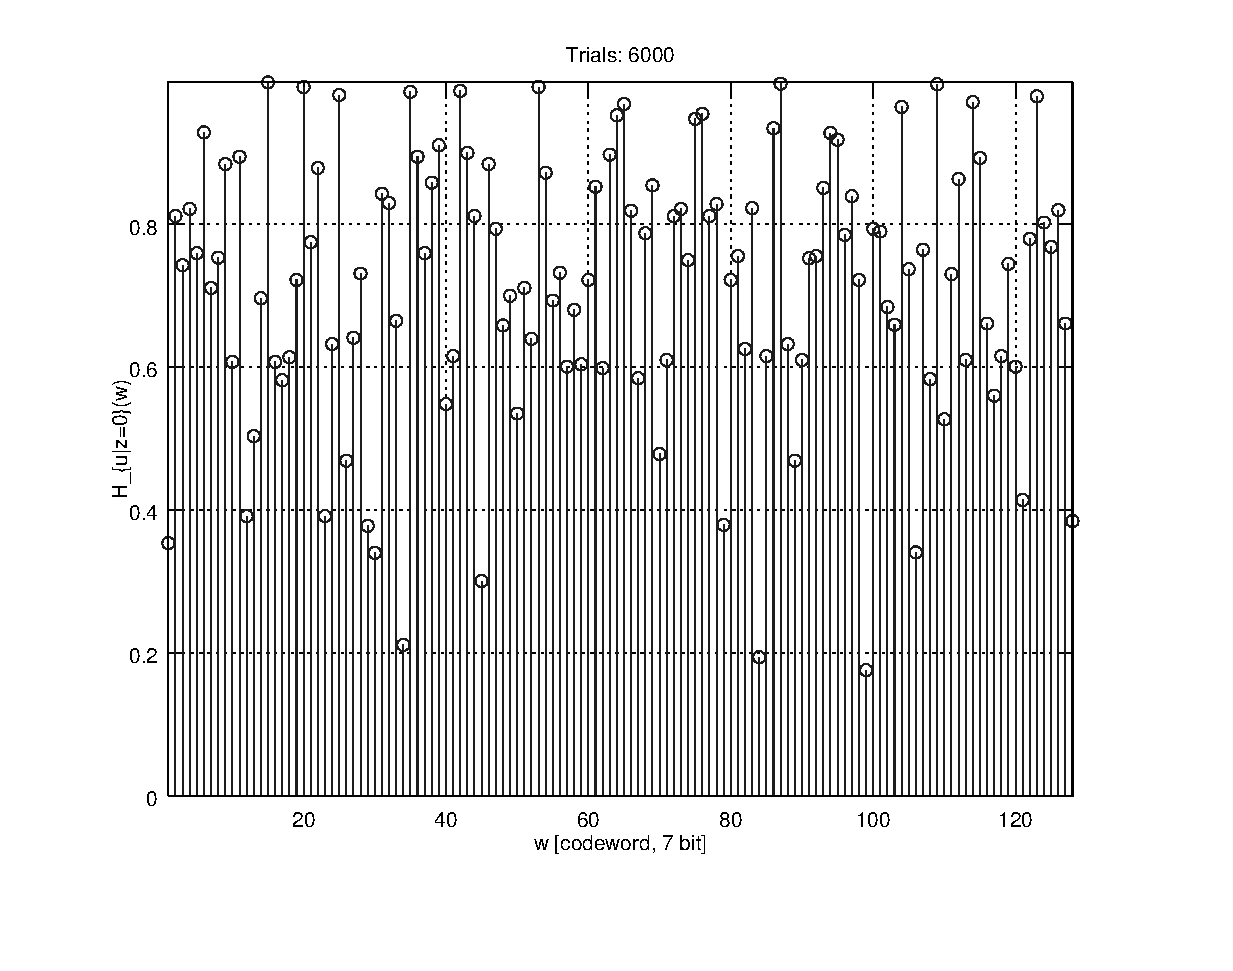
\includegraphics[scale=0.8]{bsc__0_060_0_220__6000.eps}
  \caption{$H_{u|z=0}$ for $\varepsilon_B = 0.06, \varepsilon_E = 0.22$}
  \label{fig:bsc_0.6_0.22}
\end{figure}

It can be seen that, despite transmitting at a rate lower than the overall
channel capacity, almost a whole bit leaks on average on the eavesdropper side.
Also the BER is not adequate on the eavesdropper side, as an error occurs only
in the 27.5\% of the cases. Furthermore, if we look at the plot, we see that
there are many codewords that reveal more than 2 bits to the eavesdropper;
clearly this result is not acceptable in terms of confidentiality.

Instead, reliability on the legitimate side, while not perfect, it's quite good
as we get an error in less than 4\% of the cases.

\subsection*{$R_s < C_s$: $\varepsilon_B = 0.12, \varepsilon_E = 0.38$}
Running the script gives the following result:
\begin{verbatim}
Metrics with 6000 trials:
Secrecy capacity = 0.4287
Secrecy rate     = 0.4286
BER at Bob       = 1.12e-01
BER at Eve       = 4.63e-01
-------------------------
H(u)   = 2.9989 bit
H(z)   = 6.9833 bit
H(u,z) = 9.8317 bit
H(u|z) = 2.8484 bit
H(z|u) = 6.8328 bit
I(u;z) = 0.1505 bit
\end{verbatim}

\begin{figure}[h]
  \centering
  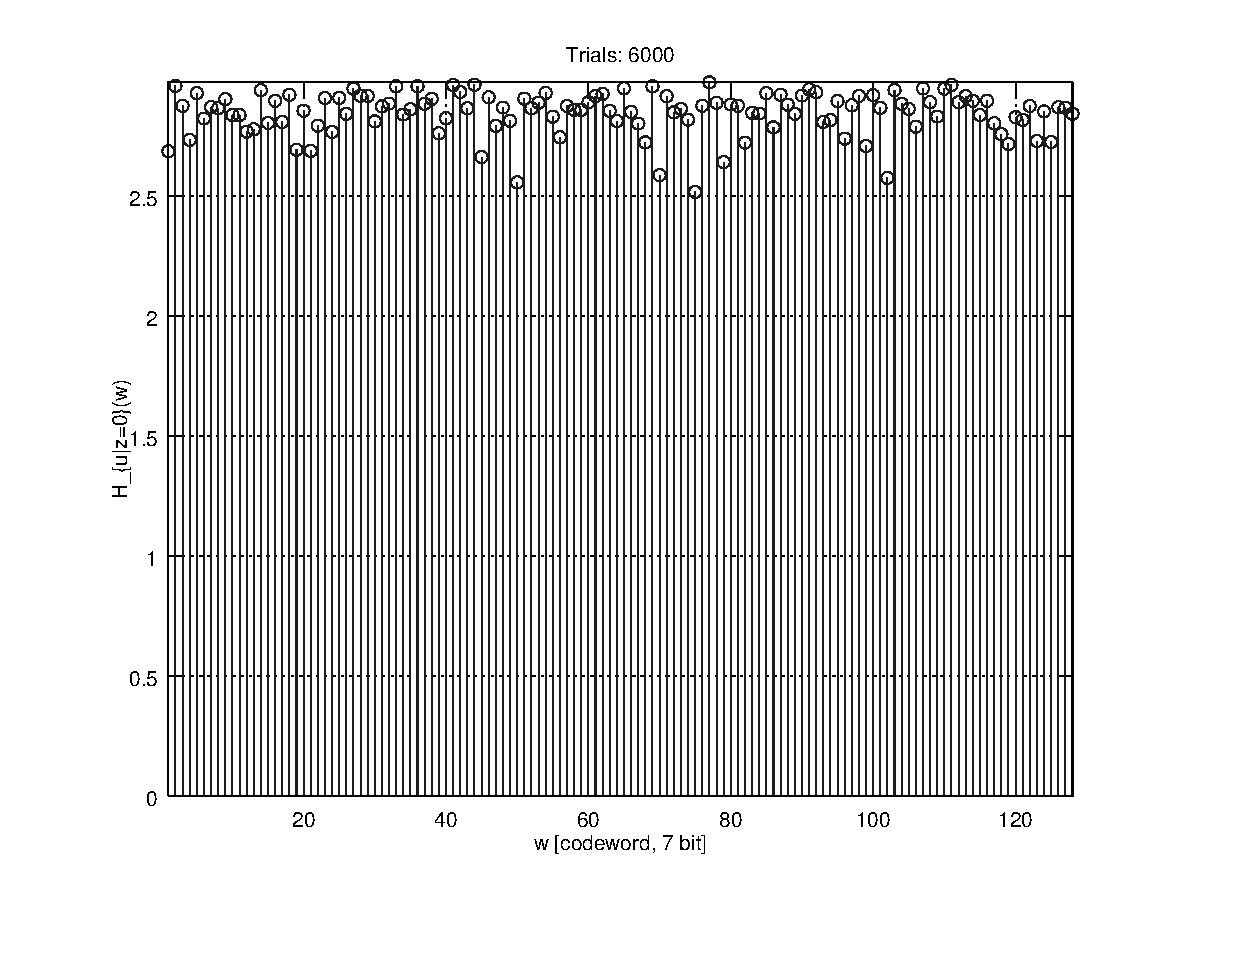
\includegraphics[scale=0.8]{bsc__0_120_0_380__6000.eps}
  \caption{$H_{u|z=0}$ for $\varepsilon_B = 0.12, \varepsilon_E = 0.38$}
  \label{fig:bsc_0.12_0.38}
\end{figure}

Despite the transmission almost fills the whole channel capacity (when in the
previous case the secrecy rate was more lower than capacity) we achieve
better results than the previous case. In particular, we almost decimated the
amount of revealed information; we can also confuse the eavesdropper more,
generating an error in more than 46\% of the times. Also the plot in
Figure~\ref{fig:bsc_0.12_0.38} shows that all eavesdropped codewords don't
retain more than 0.5 bit of mutual information with their original counterpart.

On the side of reliability, instead, things are much worse than before. In
particular, it can be noticed how, doubling the error probability on Bob we
have almost triplicated the error rate, which now is at 11\%. Given this is the
result to the net of all recoverable errors, it can be considered quite high to
consider the transmission truly "reliable".

\subsection*{$R_s > C_s$: $\varepsilon_B = 0.10, \varepsilon_E = 0.30$}
The results are:
\begin{verbatim}
Metrics with 6000 trials:
Secrecy capacity = 0.4123
Secrecy rate     = 0.4286
BER at Bob       = 8.74e-02
BER at Eve       = 3.86e-01
-------------------------
H(u)   = 2.9991 bit
H(z)   = 6.9844 bit
H(u,z) = 9.6046 bit
H(u|z) = 2.6201 bit
H(z|u) = 6.6055 bit
I(u;z) = 0.3790 bit
\end{verbatim}

\begin{figure}[h]
  \centering
  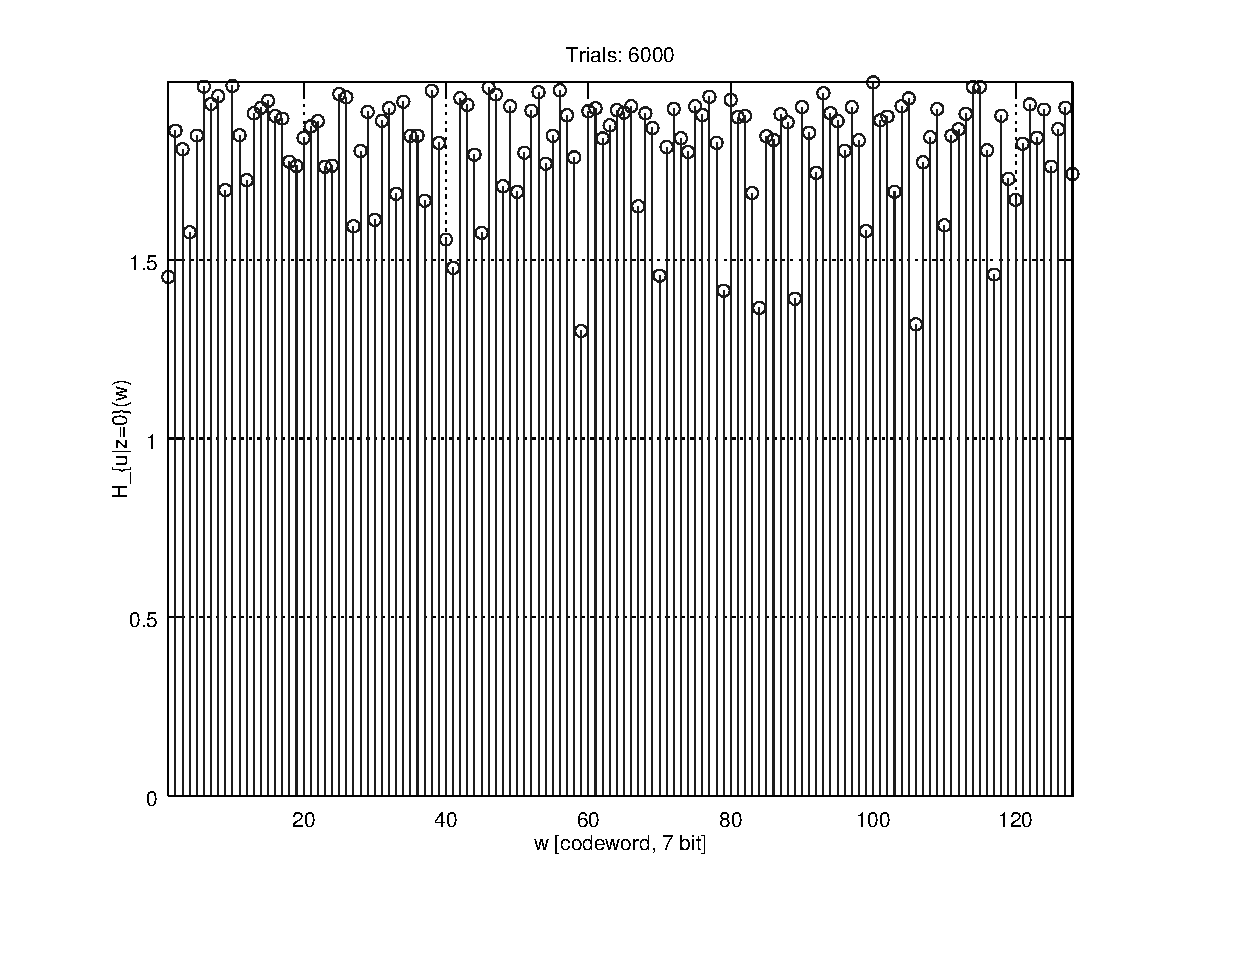
\includegraphics[scale=0.8]{bsc__0_100_0_300__6000.eps}
  \caption{$H_{u|z=0}$ for $\varepsilon_B = 0.10, \varepsilon_E = 0.30$}
  \label{fig:bsc_0.10_0.30}
\end{figure}

It is clear that we aren't achieving neither much reliability (even if better
than the previous case), nor secrecy (Figure~\ref{fig:bsc_0.10_0.30} shows that
there are codewords that leak up to a whole bit to the eavesdropper). What is
interesting, though, is the comparison of this outcome with that obtained in
the first case. In fact, despite transmitting at a secrecy rate higher than the
secrecy capacity of the channel, despite having a ratio between error
probabilities of $3$ instead of almost $4$ in the other case, we are
\emph{still} able to send more secure information than the case of
$\varepsilon_B = 0.06, \varepsilon_E = 0.22$. This points out how important is
for transmission confidentiality that the eavesdropper has a noisy channel.

\subsection*{$R_s > C_s$: $\varepsilon_B = 0.08, \varepsilon_E = 0.20$}
The results are:
\begin{verbatim}
Metrics with 6000 trials:
Secrecy capacity = 0.3197
Secrecy rate     = 0.4286
BER at Bob       = 6.12e-02
BER at Eve       = 2.47e-01
-------------------------
H(u)   = 2.9986 bit
H(z)   = 6.9236 bit
H(u,z) = 8.8099 bit
H(u|z) = 1.8863 bit
H(z|u) = 5.8114 bit
I(u;z) = 1.1123 bit
\end{verbatim}

\begin{figure}[h]
  \centering
  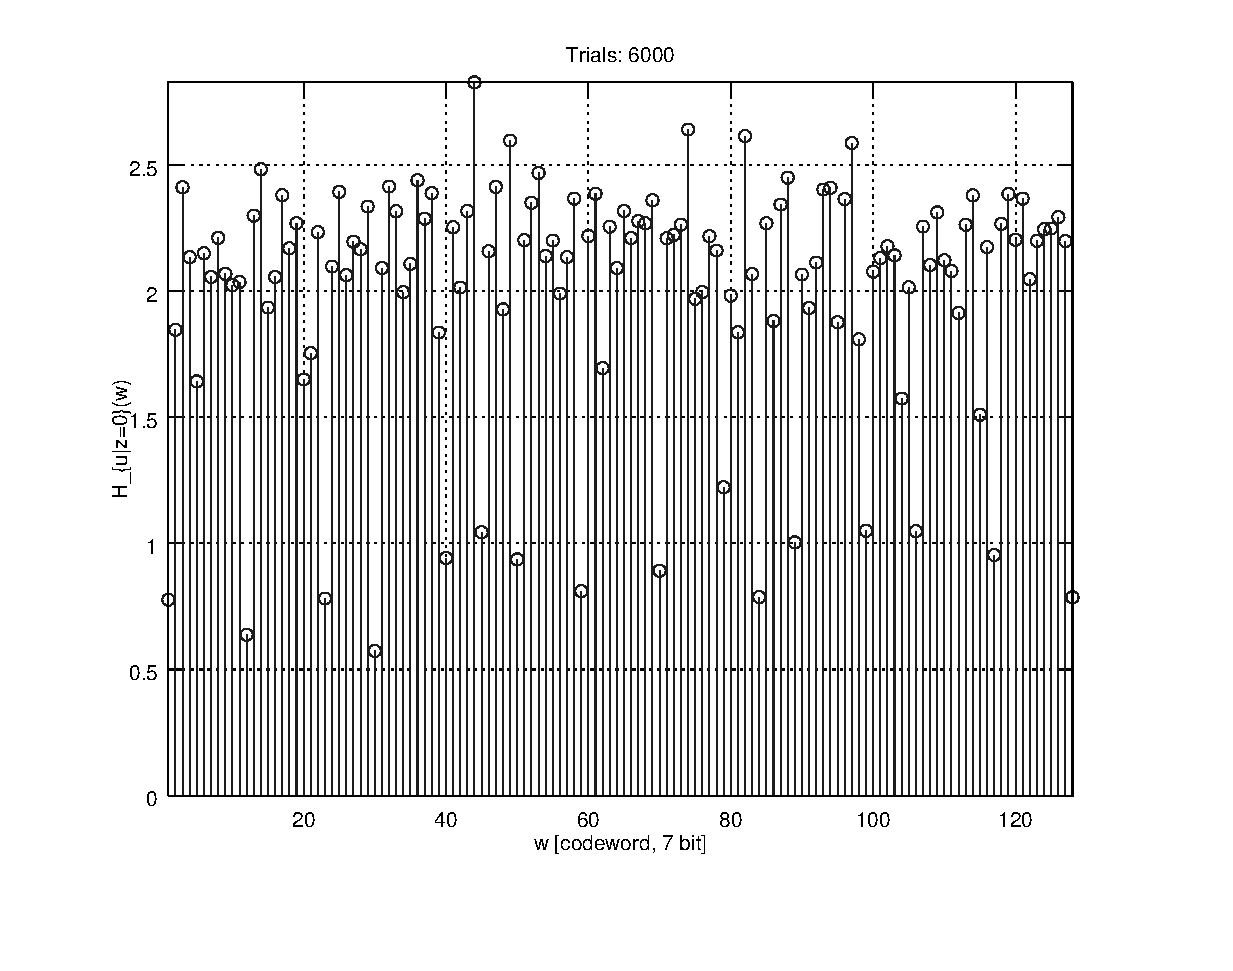
\includegraphics[scale=0.8]{bsc__0_080_0_200__6000.eps}
  \caption{$H_{u|z=0}$ for $\varepsilon_B = 0.08, \varepsilon_E = 0.20$}
  \label{fig:bsc_0.08_0.20}
\end{figure}

Here we are clearly in a bad condition. Probably the clearest evidence is
Figure~\ref{fig:bsc_0.08_0.20}, which shows how there are codewords that are
almost completely eavesdropped by Eve. As in the previous case, it's
interesting to see how, despite transmitting at $R_s \gg C_s$, the
confidentiality is not that much worse than the case of $\varepsilon_B = 0.06,
\varepsilon_E = 0.22$, again pointing out the importance of the noise level
on Eve's channel.

\subsection*{Further considerations}
We can try to see what happens in cases in which we don't achieve high secrecy
by reducing the number of secure bits transmitted. In particular, for
$\varepsilon_B = 0.06, \varepsilon_E = 0.22$, if we set $l_u = 2$ we obtain:
\begin{verbatim}
Metrics with 6000 trials:
Secrecy capacity = 0.4327
Secrecy rate     = 0.2857
BER at Bob       = 3.62e-02
BER at Eve       = 2.77e-01
-------------------------
H(u)   = 1.9997 bit
H(z)   = 6.9349 bit
H(u,z) = 8.4239 bit
H(u|z) = 1.4890 bit
H(z|u) = 6.4242 bit
I(u;z) = 0.5108 bit
\end{verbatim}

In the case $\varepsilon_B = 0.1, \varepsilon_E = 0.3, l_u = 2$, instead we
obtain:
\begin{verbatim}
Metrics with 6000 trials:
Secrecy capacity = 0.4123
Secrecy rate     = 0.2857
BER at Bob       = 8.39e-02
BER at Eve       = 3.83e-01
-------------------------
H(u)   = 1.9991 bit
H(z)   = 6.9819 bit
H(u,z) = 8.7899 bit
H(u|z) = 1.8079 bit
H(z|u) = 6.7907 bit
I(u;z) = 0.1912 bit
\end{verbatim}

We see that we're able to obtain more statistical independence between $u$ and
$z$, in both cases (almost half of mutual information as the cases with $l_u
=3$). At the same time, though, it's clear how the BER isn't much different
than before. This is evidence of what we've already stated when analyzing the
UEC: BER isn't a sufficient condition to prove perfect secrecy.

\subsection*{Conclusions}
Summing up all experimental observations, we can draw some conclusions before
moving to the case of AWGN channels.

We have seen that, as we move toward the case $\varepsilon_B = 0, \varepsilon_E
= 0.5$ we also make the channel behave as a UEC. Clearly, this is just a
theoretical result, as those error probabilities are quite unlikely to find in
practice. What happens far from these bounds is that all error patterns are
possible on both channels, but they aren't distributed uniformly. This
condition is then reflected in $\mathcal{Y}$ and $\mathcal{Z}$, and their
partitions $\{T_{y|x}\}$ and $\{T_{z|x}\}$; in particular, while both sets are
actually partitioned such that to allow perfect secrecy, the distribution of
the error patterns inside the subsets forming the partition is not uniform. It
turns out that this condition is what avoid us to obtain perfect secrecy. \\
In fact, the notion of perfect secrecy we've achieved in theory for the BSC
relies on the notion of typical sequences, which provide only an asymtptotical
result, requiring very long transmissions in order to achieve uniformity. In
our case, the combination of $l_x = 7$ and the number of simulated
transmissions is not sufficient to guarantee long term, asymptotical
uniformity.

Also, we've seen how in the case of BSCs, a fundamental condition is that of
the eavesdropper's channel being noisy. If this condition is not met, no matter
how high the secrecy capacity of the channel (i.e. how low the error
probability for the legitimate receiver), we're not able to conceal much
information. This can be seen as another way to state that high BER on the
eavesdropper side is a necessary condition for (perfect) secrecy.

\section{AWGN Channel}

Now we try to analyze the kind of secrecy achievable in a more realistic model.
We consider the case of an AWGN channel, with different SNRs at the legitimate
receiver end and at the eavesdropper end. We still consider the case of $l_x =
7, l_u = 4$ and still perform the same kind of encoding of the secret message
$u$ into the codeword $x$ by means of the \texttt{Hamming(7,4)} code. Then, we
take the codeword and perform a \textbf{128-PAM modulation} step. After that,
we simulate transmission over an AWGN channel using Matlab/Octave builtin
functions. Finally, we let both the eavesdropper and the legitimate receiver
decode the received signal.

Clearly, in this case we are not considering the transmission over a binary
medium anymore. Instead, we are dealing with a continuous signal; for this reason, we
cannot apply the information theory functions and metrics (entropy, etc.) as we
have done in the previous cases. So, the only metric we can rely upon for the
analysis is BER, which, as we've already seen, it is just a necessary condition
for (perfect) secrecy.

\subsection*{Number of transmissions}
As we've already seen in both the previous cases, BER doesn't show much
correlation with the number of transmissions over which we calculate it. So,
for this case we limit the number of observations to 2000 per model instance.
This makes each simulation faster, allowing for a broader range of trial
values.

\subsection*{Secrecy Capacity}
As we've done in the BSC case, we can derive a formulation of the secrecy
capacity as a function of $\text{SNR}_B$ and $\text{SNR}_E$ and plot this
function to find interesting regions to analyze. Though, in contrast with the
other cases, here we can achieve (at least theoretically) unconstrained secrecy
capacity. This can be seen at first by looking at the expression for $C_s$:
\[
  C_s = \frac{1}{2} [ \log_2(1+\Lambda_B) - \log_2(1+\Lambda_E) ]
\]
that is, if we let $\Lambda_B$ increase and $\Lambda_E$ decrease, the function
will increase without bound. \\
For practical reasons, we'll limit our analysis within $0$ and $50 \text{ dB}$.

That said, using the expression above for secrecy capacity, we can see how it
evolves with respect to $\Lambda_B$ and $\Lambda_E$ in
Figure~\ref{fig:awgn_mesh_cs}.

\begin{figure}[p]
  \centering
  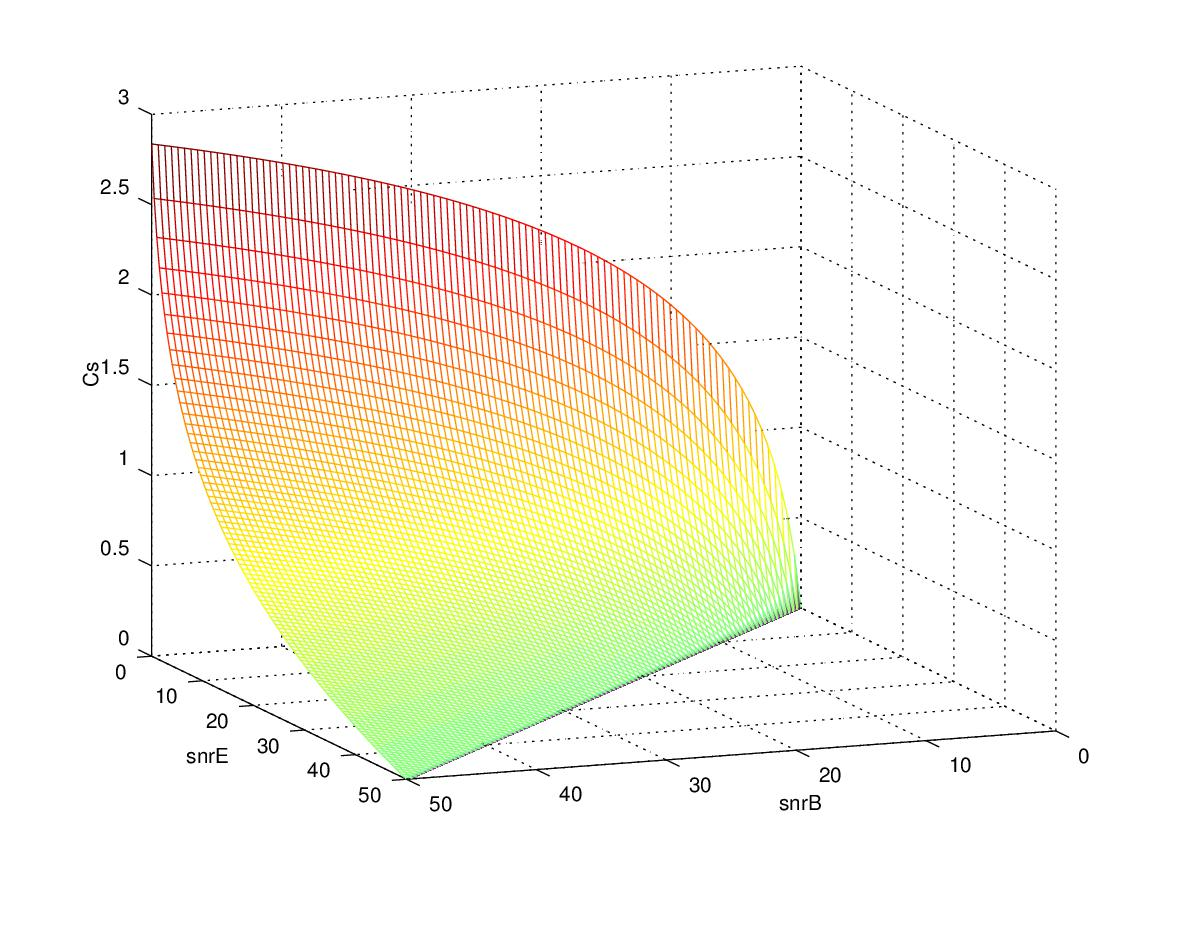
\includegraphics[scale=0.8]{awgn_mesh_cs.jpg}
  \caption{Evolution of secrecy capacity as a function of
  $\Lambda_B$ and $\Lambda_E$}
  \label{fig:awgn_mesh_cs}
\end{figure}

\end{document}
